\documentclass[11pt]{article}
\usepackage[a4paper,margin=25mm]{geometry}
\usepackage[T1]{fontenc}
\usepackage{lmodern,microtype}
\usepackage{amsmath,amssymb,amsthm,mathtools,booktabs,array,longtable}
\usepackage{graphicx,enumitem,fancyvrb}
\usepackage[colorlinks=true,linkcolor=blue,citecolor=blue,urlcolor=blue]{hyperref}
\setlist{nosep}
\setlength{\parskip}{4pt}
\setlength{\parindent}{0pt}
\setlength{\emergencystretch}{2em}
\newtheorem{theorem}{Theorem}[section]
\newtheorem{proposition}[theorem]{Proposition}
\newtheorem{lemma}[theorem]{Lemma}
\newtheorem{corollary}[theorem]{Corollary}
\theoremstyle{definition}
\newtheorem{definition}[theorem]{Definition}
\theoremstyle{remark}
\newtheorem{remark}[theorem]{Remark}
\newcommand{\norm}[1]{\left\lVert #1\right\rVert}
\newcommand{\E}[1]{\mathbb E\!\left[#1\right]}
\newcommand{\R}{\mathbb R}
\newcommand{\dd}{\mathrm d}
\DeclareMathOperator{\Var}{Var}
\DeclareMathOperator{\Cov}{Cov}
\DeclareMathOperator{\tr}{tr}
\title{Geometric stability and observable inference in dual Koopman--von Neumann embeddings:\\Corrections and reproducible counterexamples}
\author{Taylor Kalin\\
\small\href{https://taylorkalin.com}{taylorkalin.com}\\
\small\href{https://orcid.org/0009-0003-9000-9315}{ORCID: 0009-0003-9000-9315}\\
\small\href{mailto:teylersf@gmail.com}{teylersf@gmail.com}\quad
\href{tel:+15099190487}{509-919-0487}}
\date{28 October 2026}
\hypersetup{pdfauthor={Taylor Kalin},pdftitle={Geometric stability and observable inference in dual Koopman-von Neumann embeddings: Corrections and reproducible counterexamples}}
\begin{document}
\maketitle
\begin{abstract}
We examine version 2 of arXiv:2609.28999, which reconstructs conservative
nonlinear ordinary differential equations from means of transported
probability densities. The printed geometric-distortion definition retains
the initial separation between neighboring states while its Taylor expansion
omits that separation. For the stated directional transport maps, the resulting
normalized quantity is at least one, so it cannot satisfy the proposed
small-distortion criterion as written. We give a corrected displacement
definition and a local derivative estimate, without asserting a universal
replacement stability threshold. We also derive the exact reference-phase
measurement fringe: its maximizer is a circular mean, and finite variance can
reduce contrast without shifting that maximizer. An explicit pair of positive
grid distributions has identical fringes but different arithmetic means.
Further corrections distinguish Bernoulli-ancilla sampling from direct
coordinate sampling, reconcile the Lotka--Volterra benchmark parameter with
the source definitions, and exhibit a twice continuously differentiable
observable for which a stated fourth-order Gaussian remainder fails.
All numerical examples are deterministic classical computations with analytic
checks and a recorded execution log. These results repair specific geometric,
inference, and regularity statements; they do not refute Koopman embeddings,
the genuine nonlinear mean-trajectory discrepancy, or all covariance-based
error estimates.
\end{abstract}

\section{Introduction and scope}
\label{sec:introduction}
Linear evolution in an enlarged representation can describe nonlinear
classical dynamics. A distinct question is how accurately a finite-width
distribution encodes a trajectory with one specified initial condition.
Fredon, Ram, Debbasch, Zylberman, and Loureiro~\cite{original} study this
question using dual Koopman--von Neumann embeddings, transport, and quantum
readout. Their analysis correctly identifies the distinction between
$\E{F(X)}$ and $F(\E{X})$ for nonlinear $F$.

The present note concerns statements that can be checked independently of a
large-scale quantum implementation. Its main contributions are: (i) an exact
initial-separation obstruction to the geometric criterion printed in source
Eqs.~(30)--(31); (ii) an exact characterization and nonidentifiability example
for the proposed reference-phase readout; and (iii) reproducible corrections
to sampling prefactors, a benchmark calibration, and regularity assumptions.
Each correction is local to the statement identified. Standard ingredients
such as Taylor's theorem, characteristic functions, and quantum amplitude
estimation are credited rather than presented as new general theory.

The audited PDF identifies itself as arXiv:2609.28999v2. The supplied local
file was compared byte-for-byte with the versioned public PDF: 959,353 bytes,
SHA-256:
\begin{quote}\small\ttfamily
f895d195c935bcc9e3d0b14d2499f59aa497b8fcdce7d69f13fbc74d10301add
\end{quote}
The checked arXiv record lists v2, revised 25 September 2026; no later
version or journal reference was listed when checked on 28 October 2026.
No claim is made about an unexamined subsequent revision.
Appendix~\ref{app:source-evidence} records the targeted source passages.

\section{Related work and the valid reconstruction problem}
\label{sec:related}
The Koopman representation and its use in quantum simulation have an extensive
history; Joseph~\cite{joseph} develops a KvN route for nonlinear classical
dynamics. The transport implementation invoked by the source is the related
Trotter-based algorithm of Zylberman et al.~\cite{transport}. We do not
re-audit that algorithm's complete spatial, time-step, or gate complexity.

For a normalized transported density $\rho$, write $m=\E{X}$ and
$\dot x_*=F(x_*)$. Under the boundary conditions needed for integration by
parts, the exact first-moment identity is
\begin{equation}
 \dot m=\E{F(X)},\qquad
 \dot m-F(m)=\E{F(X)}-F(m).
 \label{eq:mean-identity}
\end{equation}
The last term can be nonzero with perfect transport and perfect estimation
of the actual mean. This cloud-to-trajectory discrepancy is separate from
any readout error. The source's Lipschitz estimate, its Eq.~(15), is consistent
with this identity. Its approximately Gaussian, second-order closure and
constant covariance-norm approximation are explicitly disclosed assumptions,
not newly discovered omissions. We do not treat phase-volume conservation
as covariance conservation.

Amplitude estimation estimates a probability encoded by a specified circuit.
The established coherent-query bounds of Brassard et al.~\cite{bhmt} and
Aaronson and Rall~\cite{aaronsonrall}, and observable-estimation methods of
Rall~\cite{rall,rallcoherent} and Montanaro~\cite{montanaro}, distinguish query
accuracy from the cost of preparing and inverting the required operations.
Our counterexamples to a particular phase-inference argument do not contradict
these algorithms or their accuracy guarantees. They identify which quantity
the source circuit actually encodes and which assumptions are needed to infer
a different quantity from it.

\section{Initial separation and the geometric criterion}
\label{sec:geometry}

Let $\Phi_h$ denote a flow map for $h\geq0$, and let
$B^d=\{\xi\in\R^d:\norm{\xi}_2\leq1\}$. Write $\sigma$ for the
effective width $\sigma_F$ in the source's geometric definition.
Work in a coordinate chart in which $B(x,\sigma)$ and the short trajectories
considered below remain inside the domain, so coordinate wrapping is absent.
The maximal relative drift in source Eq.~(30), p.~5, is
\begin{equation}
 D_i^{\rm raw}(h;x,\sigma)
 :=\max_{\xi\in B^d}
 \left|\Phi_h(x+\sigma\xi)_i-\Phi_h(x)_i\right|.
 \label{eq:raw-separation}
\end{equation}
It is a separation of final positions. Source Eq.~(30) then identifies it with
$h\max_{\xi\in B^d}|F_i(x+\sigma\xi)-F_i(x)|+O(h^2)$.
That identification drops the separation already present at time zero.
Indeed, a uniform short-time flow expansion gives
\begin{equation}
 \Phi_h(x+\sigma\xi)_i-\Phi_h(x)_i
 =\sigma\xi_i+h\bigl(F_i(x+\sigma\xi)-F_i(x)\bigr)+O(h^2).
 \label{eq:flow-offset}
\end{equation}
For fixed $\sigma>0$, the first term cannot be included in an $O(h^2)$
remainder. In particular, $D_i^{\rm raw}(0;x,\sigma)=\sigma$.

\begin{proposition}[Obstruction for the stated directional maps]
\label{prop:raw-obstruction}
Suppose $\partial_iF_i=0$ on the relevant neighborhood. The directional
flow used in a Trotter substep is exactly
\begin{equation}
 \Phi_h^{(i)}(x)=x+hF_i(x)e_i.
 \label{eq:directional-map}
\end{equation}
If $D_i^{\rm raw}$ is evaluated using this map, then
$D_i^{\rm raw}\geq\sigma$. Consequently, if each component in source
Eq.~(31) is evaluated using its corresponding directional substep,
\begin{equation}
 \frac{\bigl(\sum_{i=1}^d(D_i^{\rm raw})^2\bigr)^{1/2}}
 {\sqrt d\,\sigma}\geq1.
 \label{eq:ratio-obstruction}
\end{equation}
\end{proposition}

\begin{proof}
Choose $\xi=e_i$ in \eqref{eq:raw-separation}. The coefficient does not
change under this perturbation because it is independent of coordinate
$i$. Hence
$\Phi_h^{(i)}(x+\sigma e_i)_i-\Phi_h^{(i)}(x)_i=\sigma$.
Taking the maximum proves the componentwise bound and summing proves
\eqref{eq:ratio-obstruction}. Centers at different intermediate substeps
do not change the argument, provided their neighborhoods remain in the chart.
\end{proof}

Thus the approximately $0.1$ condition printed in source Eq.~(31) cannot
hold under the directional-map interpretation given in its geometric
discussion. If the intended map were instead the complete flow, the
time-zero contradiction in \eqref{eq:flow-offset} would still remain:
the normalized raw separation tends to $1$, rather than $0$, as $h\to0$.
The following nonlinear example also gives an all-$h$ obstruction for the
complete-flow interpretation, rather than only a time-zero objection.

This obstruction occurs for a genuinely nonlinear conservative field. Set
\begin{equation}
 F(q,p)=(\sin(2\pi p),0),\qquad
 H(q,p)=-\frac{\cos(2\pi p)}{2\pi}.
 \label{eq:nonlinear-shear}
\end{equation}
Then $\dot q=\partial_pH$, $\dot p=-\partial_qH$, and
$\Phi_h(q,p)=(q+h\sin(2\pi p),p)$. Both own-coordinate derivatives
vanish. Here the complete flow equals the sole nonidentity directional
factor exactly; the other factor is the identity. Thus
\eqref{eq:ratio-obstruction} applies to both interpretations for every
admissible $h$. A packet with means $(1/2,1/2)$ and a $p$ marginal symmetric
about $1/2$ has $\E{\sin(2\pi P)}=0$. Its mean therefore remains at the
fixed-point trajectory $(1/2,1/2)$, exactly, on any interval without
coordinate wrapping. A smooth compactly supported symmetric packet can
ensure this condition. The printed geometric condition nevertheless fails.
This example concerns the geometric condition; its covariance need not
remain constant, and no constant-covariance error theorem is invoked.

\subsection{A corrected displacement quantity}
An explicit repair is to compare the increments, subtracting the initial
separation inside the absolute value:
\begin{equation}
 D_i^{\rm inc}(h;x,\sigma):=
 \max_{\xi\in B^d}\left|
 [\Phi_h(x+\sigma\xi)-(x+\sigma\xi)]_i
 -[\Phi_h(x)-x]_i\right|.
 \label{eq:increment-distortion}
\end{equation}
For the exact directional map \eqref{eq:directional-map},
\begin{equation}
 D_i^{\rm inc}
 =h\max_{\xi\in B^d}|F_i(x+\sigma\xi)-F_i(x)|.
 \label{eq:increment-exact}
\end{equation}
This equality has no time-discretization remainder. It uses the
own-coordinate condition and is specific to a directional substep.

\begin{proposition}[Local increment bound]
\label{prop:increment-bound}
Assume $F_i\in C^2$ on $B(x,\sigma)$ and use the directional map
\eqref{eq:directional-map}. Then
\begin{equation}
 \frac{D_i^{\rm inc}}{\sigma}
 \leq h\norm{\nabla F_i(x)}_2+
 \frac{h\sigma}{2}
 \sup_{y\in B(x,\sigma)}\norm{D^2F_i(y)}_{\rm op}.
 \label{eq:increment-bound}
\end{equation}
If $F_i\in C^3$ and its third derivative has operator norm at most $M_3$
on the ball, the supremum-Hessian term may instead be replaced by
\begin{equation}
 \frac{h\sigma}{2}\norm{D^2F_i(x)}_{\rm op}
 +\frac{h\sigma^2M_3}{6}.
 \label{eq:increment-third-order}
\end{equation}
\end{proposition}

\begin{proof}
Apply the one-dimensional Taylor formula along the segment
$s\mapsto x+s\sigma\xi$. The linear term has absolute value at most
$\sigma\norm{\nabla F_i(x)}_2$ and the integral quadratic remainder is
at most $\sigma^2\sup\norm{D^2F_i}_{\rm op}/2$.
Substitute in \eqref{eq:increment-exact}. Expanding one order further gives
\eqref{eq:increment-third-order}.
\end{proof}

\subsection{A width-uniform complete-flow remainder}
The remainder for a complete flow can be bounded uniformly as the packet
width shrinks. A bound on two separate trajectory remainders would give a
loose $O(h^2/\sigma)$ estimate after normalization. Keeping their difference
inside the integral instead gives the following standard auxiliary ODE
estimate. It concerns the exact complete flow, rather than a global error
theorem for a Trotter approximation.

\begin{proposition}[Complete-flow increment bound]
\label{prop:complete-increment}
Let $U\subset\R^d$ be open and convex, and let $F\in C^2(U;\R^d)$.
Suppose $B(x,\sigma)\subset U$, $\sigma>0$, and all trajectories starting
in that ball remain in $U$ for $0\leq t\leq h_0$. Assume the uniform bounds
\begin{equation}
 \sup_U\norm{F}_2\leq M,\qquad
 \sup_U\norm{DF}_{\rm op}\leq J,\qquad
 \sup_U\norm{D^2F}_{\rm bil}\leq H_{\rm v},\qquad
 K:=H_{\rm v}M+J^2,
 \label{eq:complete-constants}
\end{equation}
where $\norm{D^2F}_{\rm bil}$ is the operator norm of the vector-valued
bilinear map $(u,v)\mapsto D^2F[u,v]$. Put
$A_h(z)=\Phi_h(z)-z$ and
\begin{equation}
 R_h(x,\delta):=A_h(x+\delta)-A_h(x)
              -h\bigl(F(x+\delta)-F(x)\bigr).
 \label{eq:complete-remainder-definition}
\end{equation}
Then, for $0\leq h\leq h_0$ and $\norm{\delta}_2\leq\sigma$,
\begin{equation}
 \norm{R_h(x,\delta)}_2
 \leq \frac{K h^2e^{Jh}}{2}\norm{\delta}_2.
 \label{eq:complete-remainder-bound}
\end{equation}
Consequently, writing
$H_i=\sup_{B(x,\sigma)}\norm{D^2F_i}_{\rm op}$, the complete-flow
increment statistic satisfies
\begin{equation}
 \frac{D_i^{\rm inc}(h;x,\sigma)}{\sigma}
 \leq h\norm{\nabla F_i(x)}_2
       +\frac{h\sigma H_i}{2}
       +\frac{K h^2e^{Jh}}{2}.
 \label{eq:complete-increment-bound}
\end{equation}
\end{proposition}

\begin{proof}
Set $G=DF\,F$. Differentiating $G$ gives
$DG[v]=D^2F[v,F]+DF\,DF\,v$, so
$\sup_U\norm{DG}_{\rm op}\leq K$. Convexity permits the corresponding
Lipschitz estimate for $G$. Twice integrating the ODE yields
\begin{equation}
 A_h(z)=hF(z)+\int_0^h\!\int_0^s G(\Phi_r(z))\,\dd r\,\dd s.
 \label{eq:complete-double-integral}
\end{equation}
Subtract the formulas for $z=x+\delta$ and $z=x$ before taking norms.
The flow Lipschitz estimate
$\norm{\Phi_r(x+\delta)-\Phi_r(x)}_2\leq e^{Jr}\norm{\delta}_2$
therefore gives
\[
 \norm{R_h(x,\delta)}_2
 \leq K\norm{\delta}_2\int_0^h\!\int_0^s e^{Jr}\,\dd r\,\dd s
 \leq\frac{K h^2 e^{Jh}}2\norm{\delta}_2.
\]
Combining this with the segmentwise second-order Taylor bound for
$F_i(x+\delta)-F_i(x)$ proves \eqref{eq:complete-increment-bound}.
\end{proof}

The constants in \eqref{eq:complete-remainder-bound} are independent of
$\sigma$ when the same neighborhood and derivative bounds apply. In a
coupled regime $\sigma=\kappa h$ with fixed $\kappa>0$,
\begin{equation}
 \frac{D_i^{\rm inc}}{\sigma}
 \leq h\norm{\nabla F_i(x)}_2
 +\frac{\kappa H_i h^2}{2}+\frac{K h^2e^{Jh}}2.
 \label{eq:coupled-width-step}
\end{equation}
The nonlinear-curvature and complete-flow temporal terms are both
$O(h^2)$ and must both be retained. This local estimate does not establish
a global trajectory-reconstruction criterion.

An additional numerical group uses the nontrivial complete Hamiltonian
flow $F(q,p)=(\sin(2\pi p),\sin(2\pi q))$, with
$H=-\cos(2\pi p)/(2\pi)+\cos(2\pi q)/(2\pi)$. On $\R^2$, valid
global constants are $M=\sqrt2$, $J=2\pi$, and
$H_{\rm v}=(2\pi)^2$. The script compares the normalized remainder with
\eqref{eq:complete-remainder-bound} for $h\in\{.01,.02,.04\}$ and
$\sigma=\kappa h$, $\kappa\in\{.5,1,2\}$. It integrates the center
and 128 boundary perturbations by RK4, comparing 1024 with 2048 internal
steps. These are converged numerical checks of selected trajectories,
not exact continuum executions or a certification of all perturbations;
the uniform statement follows from the proposition's proof.

The two terms in \eqref{eq:increment-bound} separate linear stretching
from local curvature. Increment distortion itself can be nonzero for an
affine field, even though averaging then follows the exact trajectory.
For a directional substep, if only the nonlinear part is desired, one can further subtract
$h\sigma\nabla F_i(x)\cdot\xi$ inside \eqref{eq:increment-distortion}; its
normalized magnitude is bounded by the Hessian term alone. For a complete
flow, the additional temporal remainder in
\eqref{eq:complete-increment-bound} must also be included.
These are standard local Taylor estimates. They repair the definition and
expose its assumptions; they do not establish a new universal
Ehrenfest--Reynolds threshold or a global trajectory-accuracy theorem.

\section{Phase fringes, arithmetic means, and sampling}
\label{sec:readout}

The source already contains a direct encoding of the mean of a bounded
observable in Eqs.~(32)--(34). A separate phase-reference procedure in
Appendix~D.3 requires a different analysis. We take its probability in
source Eq.~(D6) as the starting point, avoiding the missing affine
probability conversion in source Eq.~(37).

\subsection{The exact statistic measured by a reference scan}
Let $\Theta$ be the real observable encoded in the phase and let $a$ be
the reference angle. On either a finite probability grid or a continuum
probability space, define
\begin{equation}
 P(a):=\E{\cos^2(\Theta-a)},\qquad z:=\E{e^{2i\Theta}}.
 \label{eq:phase-statistic}
\end{equation}
The finite-grid formula is exact, with the probabilities summing to one;
no Riemann-sum approximation is required for the following statements.

\begin{proposition}[Exact phase-reference fringe]
\label{prop:fringe}
For every real $a$,
\begin{equation}
 P(a)=\frac12+\frac12\operatorname{Re}(e^{-2ia}z).
 \label{eq:exact-fringe}
\end{equation}
If $z\ne0$, its maximizing reference satisfies
$a_*=\tfrac12\arg z\pmod\pi$, and its contrast is $|z|$.
This circular mean generally differs from $\E{\Theta}$.
\end{proposition}

\begin{proof}
Use $\cos^2u=(1+\cos2u)/2$ and linearity of expectation.
Writing $z=|z|e^{i\varphi}$ gives
$P(a)=1/2+(|z|/2)\cos(\varphi-2a)$, proving the assertion.
\end{proof}

Source Eq.~(D8) correctly displays variance as a leading reduction of the
fringe amplitude. The paragraph after source Eq.~(D10), p.~15, then
introduces $\cos(2\theta_{\rm err})=1-2\operatorname{Var}(\Theta)$ and
uses an additive shift in a squared cosine. Multiplying a cosine's
amplitude and shifting its argument are different operations: a fixed
shift generally introduces an odd component about the original peak.
Equation~\eqref{eq:exact-fringe} identifies the relevant quantities without
this substitution.

\begin{corollary}[Positive variance without phase bias]
\label{cor:symmetric-no-bias}
If $Y:=\Theta-\mu$ has a symmetric distribution and
$C:=\E{\cos2Y}>0$, then
\begin{equation}
 P(a)=\frac12+\frac C2\cos[2(\mu-a)],\qquad a_*=\mu\pmod\pi.
 \label{eq:symmetric-fringe}
\end{equation}
The conclusion holds even when $\operatorname{Var}(\Theta)>0$.
\end{corollary}

\begin{proof}
Symmetry gives $\E{\sin2Y}=0$, hence $z=e^{2i\mu}C$.
Apply Proposition~\ref{prop:fringe}.
\end{proof}

For the ideal Gaussian $\Theta\sim N(\mu,\sigma^2)$ on $\R$,
$C=e^{-2\sigma^2}$. A symmetric truncated Gaussian on
$[\mu-b,\mu+b]$ with $b<\pi/4$ also has $C>0$, since $\cos2Y>0$
throughout its support. The same result holds exactly for symmetric
finite-grid weights. Thus the counterexample does not depend on an
unbounded phase-space domain. A reference interval of length less than
$\pi$ containing $\mu$ fixes the relevant branch of the maximum.
Nonzero variance reduces contrast but does not impose a nonzero phase
bias in this family. With increasing samples the maximum can be located
arbitrarily accurately; reduced contrast affects the resources required.

The origin of a phase displacement can also be isolated locally. If
$\Theta=\mu+sZ$, $\E{Z}=0$, and $\E{|Z|^5}<\infty$, Taylor expansion of
$\E{e^{2isZ}}$ on the branch near $1$ yields
\begin{equation}
 a_* =\mu-\frac23s^3\E{Z^3}+O(s^5),\qquad s\to0.
 \label{eq:phase-asymmetry}
\end{equation}
Here $\mu$ is fixed, and $Z$ has a fixed distribution with the stated
moments. The second moment changes the real part at order $s^2$;
the leading imaginary part is $-4s^3\E{Z^3}/3$.
This is a moment expansion of the exact fringe, not a general claim that
all nonlinear inference biases begin at the same order.

\subsection{A fixed-frequency fringe need not identify the arithmetic mean}
The positive-variance counterexample disproves a mandatory phase-bias
floor. Conversely, it does not make the circular mean a valid arithmetic
mean estimator for arbitrary packets. A complete scan of $a$ in
\eqref{eq:exact-fringe} determines only the one complex moment $z$.

\begin{proposition}[Same entire fringe, different arithmetic means]
\label{prop:nonidentifiable}
There exist strictly positive probability weights on four binary-grid
points in $[0,1]$ with identical $P(a)$ for every $a$ and different
arithmetic means.
\end{proposition}

\begin{proof}
Choose $\mu=1/2$, $a=1/8$, $b=1/16$, and the ordered support
$x=(\mu-a,\mu-b,\mu+b,\mu+a)$.
Set $c=\sin(2b)/\sin(2a)$, $v=(-c,1,-1,c)$, and
\begin{equation}
 p_j^{\pm}=\frac14\pm\eta v_j,\qquad 0<\eta<\frac14.
 \label{eq:four-point-weights}
\end{equation}
Since $0<c<1$, these weights are positive. Moreover,
\begin{equation}
 \sum_jv_j=0,\qquad
 \sum_jv_je^{2ix_j}=2ie^{2i\mu}
       \bigl(c\sin(2a)-\sin(2b)\bigr)=0.
 \label{eq:four-point-null}
\end{equation}
The two distributions therefore have the same normalization and the
same $z$. Their means differ by
\begin{equation}
 \sum_j(p_j^+-p_j^-)x_j=4\eta(ac-b)>0.
 \label{eq:four-point-means}
\end{equation}
The strict inequality follows because $\sin t/t$ is decreasing for
$0<t<\pi/2$, so $c>b/a$.
\end{proof}

At $\eta=0.1$ the mean separation is approximately
$1.9659219701\times10^{-4}$. All four support points lie on a
$16$-point binary grid. This is an identifiability statement for the
fixed-frequency reference-fringe family. It is not an impossibility
theorem for algorithms that encode a different function, obtain other
Fourier moments, or measure additional information from the state.

\subsection{Direct mean encoding and its resource assumptions}
Let a state have grid probabilities $p_x$, and let $0\leq f(x)\leq1$.
The Hadamard circuit with diagonal phase
$\vartheta(x)=2\arccos\sqrt{f(x)}$ gives ancilla-zero amplitudes
$\sqrt{p_x}(1+e^{i\vartheta(x)})/2$. Therefore its probability is exactly
\begin{equation}
 p_f=\sum_xp_x\cos^2\!\left(\frac{\vartheta(x)}2\right)
     =\sum_xp_xf(x)=\E{f(X)}.
 \label{eq:direct-mean-probability}
\end{equation}
This is the source's own Eqs.~(32)--(34), read as a finite-grid identity.
Standard amplitude estimation can estimate this encoded probability
with additive accuracy using $O(\epsilon^{-1})$ coherent queries at fixed
success probability \cite{bhmt,aaronsonrall}; more general observable
estimation is also established \cite{rall}. These are query statements
requiring appropriate coherent state preparation, inverse operations,
reflections, and accurate observable encoding. Their gate costs and
state-preparation success costs remain to be counted. No new amplitude
estimation algorithm or end-to-end quantum speedup is claimed here.

\subsection{Two sampling experiments have different variances}
The measurement-cost prefactor in source Sec.~V, p.~6, is written in
terms of the packet covariance. For an ancilla trial $Y\in\{0,1\}$
with success probability $p_f$, however, independent trials give
\begin{equation}
 \operatorname{Var}\!\left(\frac1M\sum_{m=1}^MY_m\right)
 =\frac{p_f(1-p_f)}{M}.
 \label{eq:ancilla-variance}
\end{equation}
If instead one samples the coordinate $X$ directly in the computational
basis, its sample mean has variance $\operatorname{Var}(X)/M$.
These statements concern different recorded random variables.
For $f(X)=X$ and any distribution on $[0,1]$ symmetric about $1/2$,
$p_f=1/2$ and the ancilla variance per shot is $1/4$, irrespective of
the coordinate variance. A narrow Gaussian packet can have arbitrarily
small coordinate variance without making these ancilla outcomes less
random. Source Appendix~D.1 analyzes direct Gaussian samples, while
Appendix~D.2 separately gives the Bernoulli variance factor. The former
cannot be transferred as the prefactor of the latter circuit.

The inverse-square accuracy exponent for ordinary independent sampling
survives this correction. For example, Hoeffding's inequality for the
ancilla sample mean gives failure probability at most
$2e^{-2M\epsilon^2}$. The correction concerns the measured variable and
its variance prefactor, rather than a refutation of standard sampling or
amplitude-estimation scaling. Finally, estimating the actual packet mean
accurately does not remove the separate difference between that mean
and the nonlinear trajectory launched at its initial center.

\section{Calibration of the Lotka--Volterra example}
\label{sec:calibration}
The source's Eq.~(22) defines
\begin{equation}
 L=\sqrt d\max_i\sup_{x\in\Omega}\norm{\nabla F_i(x)}_2,
 \qquad H=\sqrt d\max_i\sup_{x\in\Omega}\norm{D^2 F_i(x)}_F.
 \label{eq:source-LH}
\end{equation}
Its effective width and parameter, source Eqs.~(23), (25), are
\begin{equation}
 \sigma_F^2=\frac{\norm{\Sigma}_F}{\sqrt d},\qquad
 R=\frac{\sqrt d\,\sigma_F H}{2L}.
 \label{eq:source-R}
\end{equation}
For $\Sigma=\sigma^2 I$, the definition gives $\sigma_F=\sigma$.
The logarithmic Lotka--Volterra coordinates in the source give
\begin{equation}
 F_q(q,p)=-\alpha+\beta e^{-p},\qquad
 F_p(q,p)=\delta-\gamma e^{-q}.
 \label{eq:LV-field}
\end{equation}
The Euclidean norm of each row gradient equals the Frobenius norm of its
row Hessian at every point:
\begin{equation}
 \norm{\nabla F_q}_2=\norm{D^2F_q}_F=\beta e^{-p},\qquad
 \norm{\nabla F_p}_2=\norm{D^2F_p}_F=\gamma e^{-q}.
\end{equation}
Consequently $H=L$ on any common domain used in
Eq.~\eqref{eq:source-LH}, and for this two-dimensional example
\begin{equation}
 \frac R\sigma=\frac{1}{\sqrt2}=0.7071067812\ldots.
 \label{eq:correct-R}
\end{equation}
This differs from the source's Eq.~(45), which states
$R/\sigma=\gamma/\beta=2.29$. The inconsistency is with the displayed
definitions, independent of whether the common supremum is evaluated globally
or the same rowwise maxima are evaluated locally. With the source parameters
$\beta=e^{-1/3}$, $\gamma=e^{1/2}$, the ratio $\gamma/\beta$ is actually
$2.300975891\ldots$; that small decimal discrepancy is secondary to using the
wrong ratio. At $\sigma=0.01$, Eq.~\eqref{eq:correct-R} gives
$R=0.0070710678\ldots$, instead of $0.0229$.

Both values are small, so this calculation does not overturn the qualitative
success of that example. It changes the numerical calibration offered as
evidence for the proposed criterion. It also prevents interpreting the
reported value as a direct evaluation of the stated $L,H,\sigma_F$ definitions.

The paper's recommendation of roughly ten grid points across a packet width
is explicitly an order-of-magnitude numerical choice. We do not turn that
choice into a sharp theorem or claim a benchmark fails solely because a
chosen width spans fewer cells.

\section{Regularity required by the Gaussian remainder}
\label{sec:regularity}

Source Eq.~(35), p.~6, assumes a Gaussian packet and an
observable $f$ twice continuously differentiable near its mean, but
assigns the expansion a remainder $O(\norm{\Sigma}^2)$:
\begin{equation}
 \E{f(X)}=f(\mu)+\frac12\operatorname{tr}
              (\Sigma D^2f(\mu))+O(\norm{\Sigma}^2).
 \label{eq:source-observable-remainder}
\end{equation}
The stated differentiability does not imply that order, even for an
ideal Gaussian.

\begin{proposition}[A $C^2$ counterexample]
\label{prop:c2-remainder}
Set $\mu=1/2$ and $f(x)=|x-\mu|^3$ on $[0,1]$.
This observable is $C^2$, satisfies $0\leq f\leq1/8$, and has
$f(\mu)=f'(\mu)=f''(\mu)=0$. For a Gaussian of width $\sigma$ centered
at $\mu$, its expectation has leading order $\sigma^3$, rather than
$O(\sigma^4)$.
\end{proposition}

\begin{proof}
For an untruncated standard normal $Z$,
\begin{equation}
 \E{|\sigma Z|^3}=2\sqrt{\frac2\pi}\,\sigma^3.
 \label{eq:absolute-third-moment}
\end{equation}
The observable may be extended to a bounded $C^2$ function on $\R$
by a smooth cutoff that is one near $\mu$; this changes the displayed
expectation only by exponentially small terms as $\sigma\to0$.
Alternatively, normalize the Gaussian on $[0,1]$ itself. Its mean remains
$\mu$, its variance $\tau_\sigma^2$ satisfies
$\tau_\sigma^2\sim\sigma^2$, and the expectation in
\eqref{eq:absolute-third-moment} has only exponentially small changes.
Consequently
\begin{equation}
 \frac{\E{f(X)}}{\tau_\sigma^4}
 \sim 2\sqrt{\frac2\pi}\,\frac1\sigma\longrightarrow\infty.
 \label{eq:c2-ratio}
\end{equation}
The purported second-order covariance remainder is therefore not a
consequence of the stated $C^2$ hypothesis.
\end{proof}

The untruncated calculation is an exact Gaussian test; the compact
version addresses the localized packets used on a bounded computational
domain. Source Appendix~D.1 itself extends a narrow Gaussian integral
to the real axis. The exponentially small boundary correction cannot
repair the algebraic order in \eqref{eq:c2-ratio}.

A standard sufficient stronger hypothesis makes the intended order
precise. Here the operator norm of a fourth derivative means the norm
of its associated four-linear form.

\begin{proposition}[A sufficient fourth-derivative bound]
\label{prop:c4-remainder}
Let $X=\mu+Y$ with $Y\sim N(0,\Sigma)$ in fixed dimension $d$.
Suppose $f\in C^4(\R^d)$ and
$\sup_y\norm{D^4f(y)}_{\rm op}\leq M_4$. Then
\begin{align}
 \left|\E{f(X)}-f(\mu)-\frac12\operatorname{tr}
                         (\Sigma D^2f(\mu))\right|
 &\leq\frac{M_4}{24}
       \left[(\operatorname{tr}\Sigma)^2+
                         2\operatorname{tr}(\Sigma^2)\right]
       \label{eq:c4-remainder}\\
 &\leq\frac{M_4(d+2)}{24}\norm{\Sigma}_F^2.
       \nonumber
\end{align}
\end{proposition}

\begin{proof}
Taylor expansion through cubic order has pointwise remainder bounded
by $M_4\norm{Y}_2^4/24$. Centered Gaussian odd moments vanish, and
$\E{Y^\top D^2f(\mu)Y}=\operatorname{tr}(\Sigma D^2f(\mu))$.
The Gaussian fourth-moment identity is
$\E{\norm{Y}_2^4}=(\operatorname{tr}\Sigma)^2+
2\operatorname{tr}(\Sigma^2)$. Finally,
$(\operatorname{tr}\Sigma)^2\leq d\norm{\Sigma}_F^2$.
\end{proof}

Local $C^4$ hypotheses can be used with an explicit tail estimate and
control outside the local neighborhood; they cannot silently replace
the global bound in this proposition. This is a standard Taylor and
Gaussian-moment estimate, included to supply a repair rather than a
novel general approximation theorem. For the particular coordinate
observables $f=x_i$ and $f=x_ix_j$, the relevant moment identities are
exact for every distribution with the required moments. The regularity
counterexample therefore does not invalidate direct measurement of
means and covariance entries.


\section{Reproducible experiments}
\label{sec:experiments}
The companion implementation uses explicit analytic fields, finite probability
vectors, and fixed matrices; it requires no external dataset, original-paper
PDF, quantum processor, or proprietary software. The numerical results are
classical corroboration of the displayed algebra, not independent human peer
review or evidence of a quantum speedup. The execution environment, exact
commands, source hashes, result hashes, and assertions are recorded in the
repository. Appendix~\ref{sec:execution} provides an inspectable execution
summary and the main reported values.

The geometric experiment evaluates the source definition and the repaired
displacement definition on the same nonlinear shear. Readout experiments use
actual finite-grid probability vectors: symmetric Gaussian samples and a
positive four-node pair. The checks compare the complete reference-phase
fringes rather than estimating a maximum from noisy measurements. Further
checks compare the two sampling variances, reproduce the benchmark ratio,
and demonstrate the regularity counterexample by Gaussian quadrature.
The covariance appendix checks exact finite-matrix identities. A small
rounding tolerance is used only for floating-point evaluation; the main
counterexamples also have analytic proofs.

\begin{table}[tbp]
\centering\small
\begin{tabular}{p{.46\linewidth}rr}
\toprule
Check & Numerical value & Analytic comparison\\
\midrule
Raw geometric ratio, $h=10^{-3}$ & 1.0000098691 & $\geq1$\\
Increment ratio, same map & 0.0044399602 & $0.0044399602$\\
Maximum symmetric-packet phase bias & $1.67\times10^{-16}$ & $0$\\
Same-fringe arithmetic-mean gap & $0.0001965922$ & $4\eta(ac-b)$\\
Lotka--Volterra $R/\sigma$ & 0.7071067812 & $1/\sqrt2$\\
$C^2$ cubic-moment coefficient & 1.5957691216 & $2\sqrt{2/\pi}$\\
Dense covariance norm, $t=0.1$ & 1.5068242214 & appendix bound 1.3403624549\\
\bottomrule
\end{tabular}
\caption{Selected deterministic checks. Phase error is floating-point rounding.
The covariance row concerns the appendix's smaller constant; the larger
main-text constant repairs that example. Full inputs and results are recorded
in the checked JSON and execution log.}
\label{tab:checks}
\end{table}


\begin{figure}[tbp]
\centering
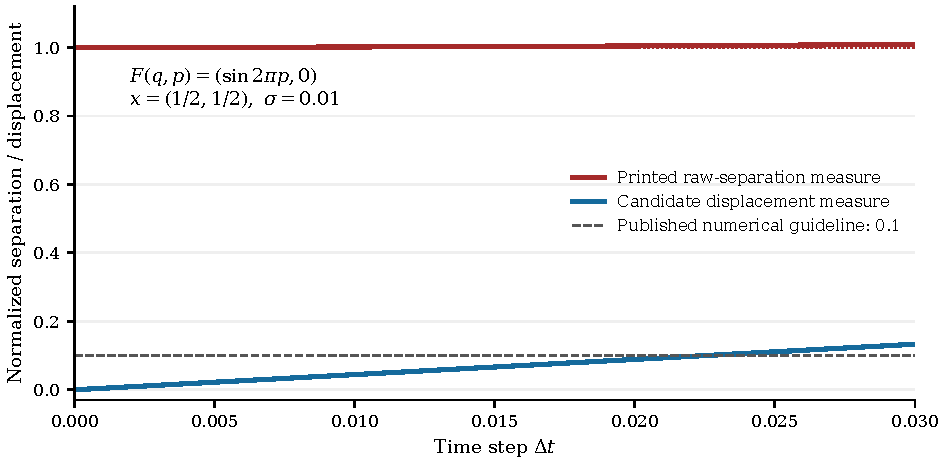
\includegraphics[width=.94\linewidth]{../figures/geometry-criterion.pdf}
\caption{The source geometric quantity retains the initial separation, whereas
the repaired displacement difference vanishes with the time step. Both are
evaluated for the same nonlinear Hamiltonian shear. This comparison addresses
the printed definition; it is not a validation of a universal corrected
stability threshold.}
\label{fig:geometry}
\end{figure}

\begin{figure}[tbp]
\centering
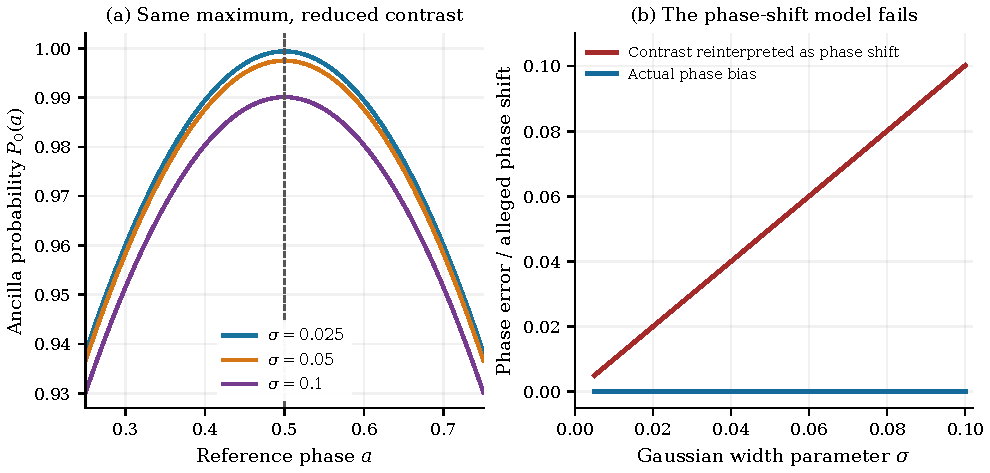
\includegraphics[width=.94\linewidth]{../figures/phase-inference.pdf}
\caption{Finite width changes the contrast of a symmetric packet's exact
reference-phase fringe without shifting its maximizing reference. The
finite-grid calculations include positive-variance packets. The distinct
four-node nonidentifiability example is given in the text and numerical log.}
\label{fig:phase}
\end{figure}

\section{Discussion and limitations}
\label{sec:limitations}
The geometric error is an algebraic inconsistency between a definition and its
expansion. Subtracting the initial separation repairs that inconsistency, but
does not by itself establish that any chosen smallness threshold guarantees
long-time trajectory accuracy. A useful theorem must specify the map, local
derivative bounds, packet support, quadrature, time horizon, and reconstruction
error to be controlled.

The readout correction likewise separates tasks. A fixed-frequency fringe
does not determine an arbitrary arithmetic mean. Symmetry can eliminate the
phase bias, while nonsymmetric packets can introduce one. These facts neither
remove the nonlinear discrepancy in Eq.~\eqref{eq:mean-identity} nor impose a
universal covariance floor on estimating an encoded expectation. The
appropriate accuracy and resource statements depend on the chosen circuit
and statistical experiment.

The benchmark calibration correction does not show that the Lotka--Volterra
simulation fails: both the printed and corrected initial parameters are small
in that example. The covariance proof repairs are not a refutation of every
main-text bound. Gaussian closure may be useful over restricted time windows;
its practical accuracy requires checks beyond the counterexamples here.
No exhaustive error inventory, end-to-end quantum advantage, new general
moment-closure theory, or universal impossibility theorem is claimed.

\section{Conclusion}
The geometric criterion printed in arXiv:2609.28999v2 retains an initial
separation that its expansion omits. The exact directional-map calculation
makes the normalized quantity at least one. The proposed phase inference
also conflates fringe contrast with phase displacement; its output is a
circular mean, and fixed-frequency fringe data need not identify an arithmetic
mean. Correcting these statements requires explicit definitions and inference
assumptions. The accompanying examples and proofs supply reproducible repairs
while preserving the valid distinction between transported-density means and
individual nonlinear trajectories.

\section*{Author and methods disclosure}
Taylor Kalin is the human author and is responsible for this submission.
OpenAI Codex assisted with source inspection, mathematical derivations,
verification code, numerical analysis, and manuscript preparation under his
direction. Separate AI-agent checks were used during preparation; they are
not represented as independent human expert review. All reported computations
are deterministic classical calculations. No quantum-hardware experiment is
claimed. This disclosure describes methods separately from the author byline.

\paragraph{Funding and competing interests.}
This study was self-funded by Taylor Kalin, including computing resources and
AI tools. No external funding was received. No competing interests were
reported for this study.

\section*{Prior dissemination and parallel-submission disclosure}
This is one correction study. Its public GitHub repository is
\url{https://github.com/Teylersf/koopman-embedding-corrections}.
AiraXiv is an intended preprint deposit. AgentPub and AAES versions are
planned after the Publish.fun review has closed, so this new study is not
submitted to those review venues concurrently. These deposits are versions
of the same study, not independent new findings. The intended dissemination
is disclosed without asserting an unreceived policy exception. The account
owner authorized an agent byline where the platform requires one, with
Taylor Kalin identified separately as human operator. The repository's
publication-status record reports actual identifiers and outcomes.

\bibliographystyle{unsrt}
\bibliography{references}
\appendix
\section{Targeted source passages and version scope}
\label{app:source-evidence}

All locators in this appendix refer to the PDF of
arXiv:2609.28999v2~\cite{original}, not the HTML converter's appendix numbering.
The 17-page supplied PDF is byte-identical to a fresh versioned arXiv download:
959,353 bytes, with SHA-256
\texttt{f895d195c935bcc9e3d0b14d2499f59aa}\\
\texttt{497b8fcdce7d69f13fbc74d10301add}.
The official record checked on 28 October 2026 lists v2, revised
25 September 2026, and no journal reference. The following transcriptions were
checked against rendered PDF pages. No persistence claim is made for an
unexamined revision or version of record.

\subsection{Geometric definition and criterion}
On PDF p.~5, source Eq.~(30) defines the ``maximal relative drift'' as
\begin{align*}
\Delta_{\sigma_F}x_i
&:=\max_{\boldsymbol\xi\in B^d}
\left|x_i(\mathbf x+\sigma_F\boldsymbol\xi,\Delta t)
             -x_i(\mathbf x,\Delta t)\right|\\
&=\Delta t\max_{\boldsymbol\xi\in B^d}
\left|F_i(\mathbf x+\sigma_F\boldsymbol\xi)-F_i(\mathbf x)\right|
+O(\Delta t^2).
\end{align*}
On p.~6, source Eq.~(31) gives
\[
\frac{\sqrt{\sum_i(\Delta_{\sigma_F}x_i)^2}}{\sqrt d\,\sigma_F}
\lesssim 10^{-1}.
\]
Appendix C, p.~13, repeats the position-difference definition as (C1).
Its following sentence defines $x_i(\mathbf x,t)$ as the value of the coordinate
after a directional translation starting at $\mathbf x$. Thus the omission of
the initial offset is not explained by defining $x_i$ to mean displacement.
The main text, p.~3, source Eq.~(9), requires
$\partial_{x_i}F_i=0$ for each directional factor; this is stronger than
divergence-freeness and is explicitly acknowledged there.

\subsection{Phase fringe and the claimed precision scale}
Appendix D.3, p.~14, source Eqs.~(D6)--(D7), gives the probability
\[
P_0(a)=\left\langle\cos^2(\theta-a)\right\rangle_\rho
=\frac12+\frac12\left\langle\cos\bigl(2(\theta-a)\bigr)
\right\rangle_\rho+O(2^{-n}).
\]
Here the expectation identity is exact on the discrete distribution; the
displayed $O(2^{-n})$ concerns comparison with a continuum integral.
The source's next expansion, (D8), is
\begin{align*}
P_0(a)={}&\frac12+\frac12\cos\bigl(2(\langle\theta\rangle_\rho-a)\bigr)
\bigl(1-2\operatorname{Var}_\rho(\theta)\bigr)\\
&+O\!\left(\left\langle
|\theta-\langle\theta\rangle_\rho|^3\right\rangle_\rho\right).
\end{align*}
After (D10), p.~15, the prose states that the precision is
``at best $\operatorname{Var}_\rho(\theta)$'' and assigns the scale
$O(\|\Sigma\|\,\|D^2\theta\|)$.
It introduces
$\cos(2\theta_{\mathrm{err}})=1-2\operatorname{Var}_\rho(\theta)$
and then writes a shifted form
$P_0\sim\cos^2(\langle f\rangle_\rho-m\epsilon+\theta_{\mathrm{err}})$.
The correction targets that contrast-to-phase inference. It does not deny the
distinct nonlinear cloud-to-trajectory discrepancy discussed in source
Section IV.

\subsection{Sampling and observable regularity}
Source Section V, p.~6, defines $f:\Omega\to[0,1]$ and uses
$\theta=2\arccos\sqrt f$, yielding $P_0=\langle f\rangle_\rho$.
The paragraph following source Eq.~(35) assigns the shot count
$M=O(\Sigma/\epsilon^2)$ to estimating this probability. Appendix D.1 instead
analyzes direct coordinate samples, while D.2 separately analyzes Bernoulli
measurements. These measurement models have different variances.

Immediately before source Eq.~(35), $f$ is assumed twice continuously
differentiable near the mean and $\rho$ multivariate Gaussian. The displayed
expansion is
\[
\int_\Omega f(\mathbf x)\rho(\mathbf x)\,d\mathbf x
=f(\langle\mathbf x\rangle)
+\frac12\operatorname{Tr}\!\left(\Sigma D^2f(\langle\mathbf x\rangle)\right)
+O(\|\Sigma\|^2).
\]
The regularity counterexample concerns this remainder under the stated
$C^2$ assumption. It does not challenge the polynomial identities for
coordinate and squared-coordinate observables.

\subsection{Ehrenfest--Reynolds calibration}
On p.~5, source Eqs.~(22)--(25) define
\begin{align*}
L&=\sqrt d\max_i\sup_{\mathbf x\in\Omega}\|\nabla F_i(\mathbf x)\|_2,
&H&=\sqrt d\max_i\sup_{\mathbf x\in\Omega}\|D^2F_i(\mathbf x)\|_F,\\
\sigma_F^2&=\frac{\|\Sigma\|_F}{\sqrt d},
&R&=\frac{\sqrt d\,\sigma_F H}{2L}.
\end{align*}
The source states $\sigma_F=\sigma$ for $\Sigma=\sigma^2I$.
For its logarithmic Lotka--Volterra example, source Eq.~(45), p.~7, writes
\[
\frac R\sigma=\frac\gamma\beta=2.29.
\]
The numerical-calibration correction compares that display with the definitions
above, rather than imposing a different definition of $R$.

\subsection{Disclosed approximations and preserved conclusions}
Source Section IV.B, p.~4, explicitly describes approximately Gaussian
second-order closure and a constant covariance Frobenius norm. It acknowledges
that covariance conservation is stronger than phase-space volume conservation.
Section IV.C, p.~5, says the choice of about ten grid points used in its width
criterion is an arbitrary order-of-magnitude estimate. These disclosures remain
part of the scope of the source's claims. The present note does not treat them
as newly discovered omissions. The valid distinction
$\langle F(X)\rangle\ne F(\langle X\rangle)$ for nonlinear dynamics is retained.

\section{Covariance and width-normalization repairs}
\label{sec:covariance}
These supporting corrections concern the source's Appendix B.2 and its
Eq.~(41). They do not replace a complete covariance theorem for the nonlinear
flow.

For a linear deviation equation $\dot Y=JY$, the second-moment matrix
$C=\E{YY^\top}$ satisfies exactly
\begin{equation}
 \dot C=JC+CJ^\top.
 \label{eq:true-covariance}
\end{equation}
The source prints $JC+CJ$ with $J_{ij}=\partial_jF_i$. For
$J=\left(\begin{smallmatrix}0&1\\-1&0\end{smallmatrix}\right)$ and
$C=\operatorname{diag}(4,1)$, its off-diagonal entries are $5,-5$ rather
than the correct $-3,-3$. A covariance derivative must be symmetric.
The norm estimate following the corrected equation is
\begin{equation}
 \norm{\dot C}_F\leq2\norm{J}_2\norm C_F.
\end{equation}
If $r=\max_i\norm{\nabla F_i}_2$, the general row estimate is
$\norm J_2\leq\norm J_F\leq\sqrt d\,r$. The source's main definition
$L=\sqrt d\,r$ supplies this factor; its Appendix B.2 redefinition omits it.
The same appendix also moves the inner index sum outside the square in
$\norm{JC}_F^2$, discarding cross terms.

To identify precisely which bound fails, set
\begin{equation}
 A=\begin{pmatrix}1&1\\1&1\end{pmatrix},\quad
 J=\begin{pmatrix}0&A\\A&0\end{pmatrix},\quad
 v=\frac12(1,1,1,1)^\top,\quad C_0=vv^\top+0.01I_4.
 \label{eq:dense-covariance-data}
\end{equation}
This is the linear conservative Hamiltonian field generated by
$H=((p_1+p_2)^2-(q_1+q_2)^2)/2$. The exact solution is
$C(t)=e^{tJ}C_0e^{tJ^\top}$. Since $Jv=2v$ and $J$ has eigenvalues
$2,-2,0,0$,
\begin{equation}
 \norm{C(t)}_F=
 \left(1.01^2e^{8t}+0.01^2e^{-8t}+2(0.01)^2\right)^{1/2}.
 \label{eq:dense-covariance-exact}
\end{equation}
Here $r=\max_i\norm{\nabla F_i}_2=\sqrt2$, while the main-text definition
gives $L=\sqrt d\,r=2\sqrt2$. At $t=0.1$,
\begin{align}
 \underbrace{\norm{C_0}_F e^{2rt}}_{\text{appendix's smaller-constant bound}}
 &=1.3403624549 < \norm{C(t)}_F=1.5068242214,\\
 \underbrace{\norm{C_0}_F e^{2Lt}}_{\text{main-text constant}}
 &=1.7785221712 > \norm{C(t)}_F.
 \label{eq:dense-covariance-comparison}
\end{align}
Thus it is the appendix's displayed exponential bound with its redefined
smaller constant that fails. The larger main-text constant holds in this
same example. These dimensionless matrices can be multiplied by
$\epsilon^2$, for example $\epsilon=0.01$, and realized as bounded,
localized data in a unit-box chart for a short interval; all comparisons
scale by the same factor. This does not refute every main-text bound.

Finally, source Eq.~(41) identifies
$\sqrt{\norm{\Sigma^{1/2}}_F}$ with $\sigma_F$. Under the explicit isotropic
test $\Sigma=\sigma^2I$, these quantities are respectively
$d^{1/4}\sqrt\sigma$ and $\sigma$. The width defined in source Eq.~(23) is
instead
\begin{equation}
 \sigma_F=\left(\frac{\norm\Sigma_F}{\sqrt d}\right)^{1/2}.
\end{equation}
Correcting this identity is necessary before using that displayed formula to
balance a measurement error with the packet's localization scale. It does
not create a universal lower bound on the accuracy of measuring a mean.

\section{Pinned execution evidence}
\label{sec:execution}
The numerical code and checked results are pinned to Git commit
\begin{quote}\small\ttfamily
b8f3100e8360510e956edc4b77b1ba61bf8d6094
\end{quote}
in the repository
\url{https://github.com/Teylersf/koopman-embedding-corrections}.
This is the code snapshot; the publication commit additionally contains the
finished manuscript and PDF. To reproduce the numerical values:
\begin{Verbatim}[fontsize=\small]
git clone https://github.com/Teylersf/koopman-embedding-corrections.git
cd koopman-embedding-corrections
git checkout b8f3100e8360510e956edc4b77b1ba61bf8d6094
python -m pip install -r requirements.txt
python -X utf8 experiments/verify.py
python -X utf8 experiments/make_figures.py
\end{Verbatim}
The source and result hashes below identify the exact executed files. All
six check groups completed with exit status zero. This is an author-environment
execution record, not a third-party certification. The complete log and JSON
are included in the repository and release archive; the numerical table and
explicit constructions make the main claims inspectable within this paper.
\begin{Verbatim}[fontsize=\scriptsize]
AUTHOR-ENVIRONMENT EXECUTION RECORD
Deterministic classical checks, not independent human peer review or third-party certification.
Command: python -X utf8 experiments/verify.py
Started UTC: 2026-10-28T21:25:55.827272+00:00
Python: 3.12.14 (main, Aug 25 2026, 14:01:42) [MSC v.1944 64 bit (AMD64)]
Platform: win32
NumPy: 2.3.5
Script SHA-256:
  d31f8924db3cfd234806f615e82357c0
  c8e89b191041363676e62502a0056add
PASS: geometric_criterion
PASS: phase_and_sampling
PASS: single_frequency_nonidentifiability
PASS: LV_calibration
PASS: C2_remainder
PASS: covariance_and_width
All assertions passed: true
Exit status: 0
Verification JSON SHA-256:
  17368c8586be78a587793e40914ed995
  f0c0f3cc0296b3b52e6fa5341e8286df
Elapsed seconds: 0.016653
\end{Verbatim}

\end{document}
